% Digital Logic Report Template
% Created: 2020-01-10, John Miller

%==========================================================
%=========== Document Setup  ==============================

% Formatting defined by class file
\documentclass[11pt]{article}

% ---- Document formatting ----
\usepackage[margin=1in]{geometry}	% Narrower margins
\usepackage{booktabs}				% Nice formatting of tables
\usepackage{graphicx}				% Ability to include graphics

%\setlength\parindent{0pt}	% Do not indent first line of paragraphs 
\usepackage[parfill]{parskip}		% Line space b/w paragraphs
%	parfill option prevents last line of pgrph from being fully justified

% Parskip package adds too much space around titles, fix with this
\RequirePackage{titlesec}
\titlespacing\section{0pt}{8pt plus 4pt minus 2pt}{3pt plus 2pt minus 2pt}
\titlespacing\subsection{0pt}{4pt plus 4pt minus 2pt}{-2pt plus 2pt minus 2pt}
\titlespacing\subsubsection{0pt}{2pt plus 4pt minus 2pt}{-6pt plus 2pt minus 2pt}

% ---- Hyperlinks ----
\usepackage[colorlinks=true,urlcolor=blue]{hyperref}	% For URL's. Automatically links internal references.

% ---- Code listings ----
\usepackage{listings} 					% Nice code layout and inclusion
\usepackage[usenames,dvipsnames]{xcolor}	% Colors (needs to be defined before using colors)

% Define custom colors for listings
\definecolor{listinggray}{gray}{0.98}		% Listings background color
\definecolor{rulegray}{gray}{0.7}			% Listings rule/frame color

% Style for Verilog
\lstdefinestyle{Verilog}{
	language=Verilog,					% Verilog
	backgroundcolor=\color{listinggray},	% light gray background
	rulecolor=\color{blue}, 			% blue frame lines
	frame=tb,							% lines above & below
	linewidth=\columnwidth, 			% set line width
	basicstyle=\small\ttfamily,	% basic font style that is used for the code	
	breaklines=true, 					% allow breaking across columns/pages
	tabsize=3,							% set tab size
	commentstyle=\color{gray},	% comments in italic 
	stringstyle=\upshape,				% strings are printed in normal font
	showspaces=false,					% don't underscore spaces
}

% How to use: \Verilog[listing_options]{file}
\newcommand{\Verilog}[2][]{%
	\lstinputlisting[style=Verilog,#1]{#2}
}




%======================================================
%=========== Body  ====================================
\begin{document}

\title{ELC 2137 Lab 11: FSM: Guessing Game}
\author{Put your name(s) here}

\maketitle


\section*{Summary}

Type the summary of your experiment and results here.  


\section*{Q\&A}

Answer questions posed in the lab assignment here.


\section*{Results}

\begin{enumerate}
	
	\item Debounce Test Simulation
	
	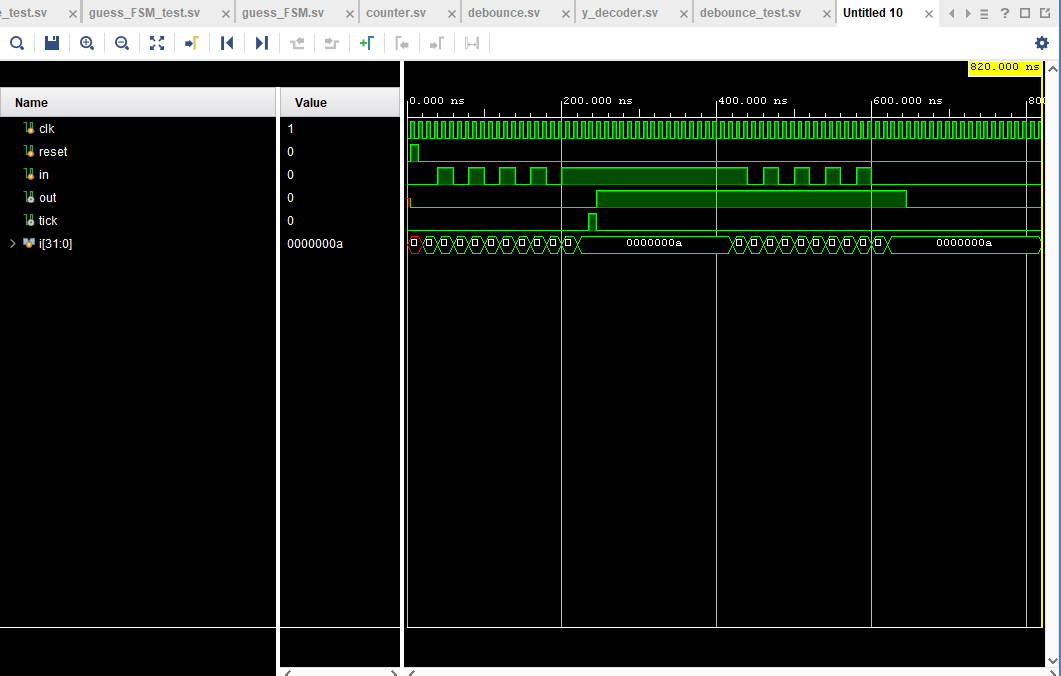
\includegraphics[width=0.8\textwidth]{debounce_sc.PNG}
	
	\item Guess FSM Test Simulation 
	
	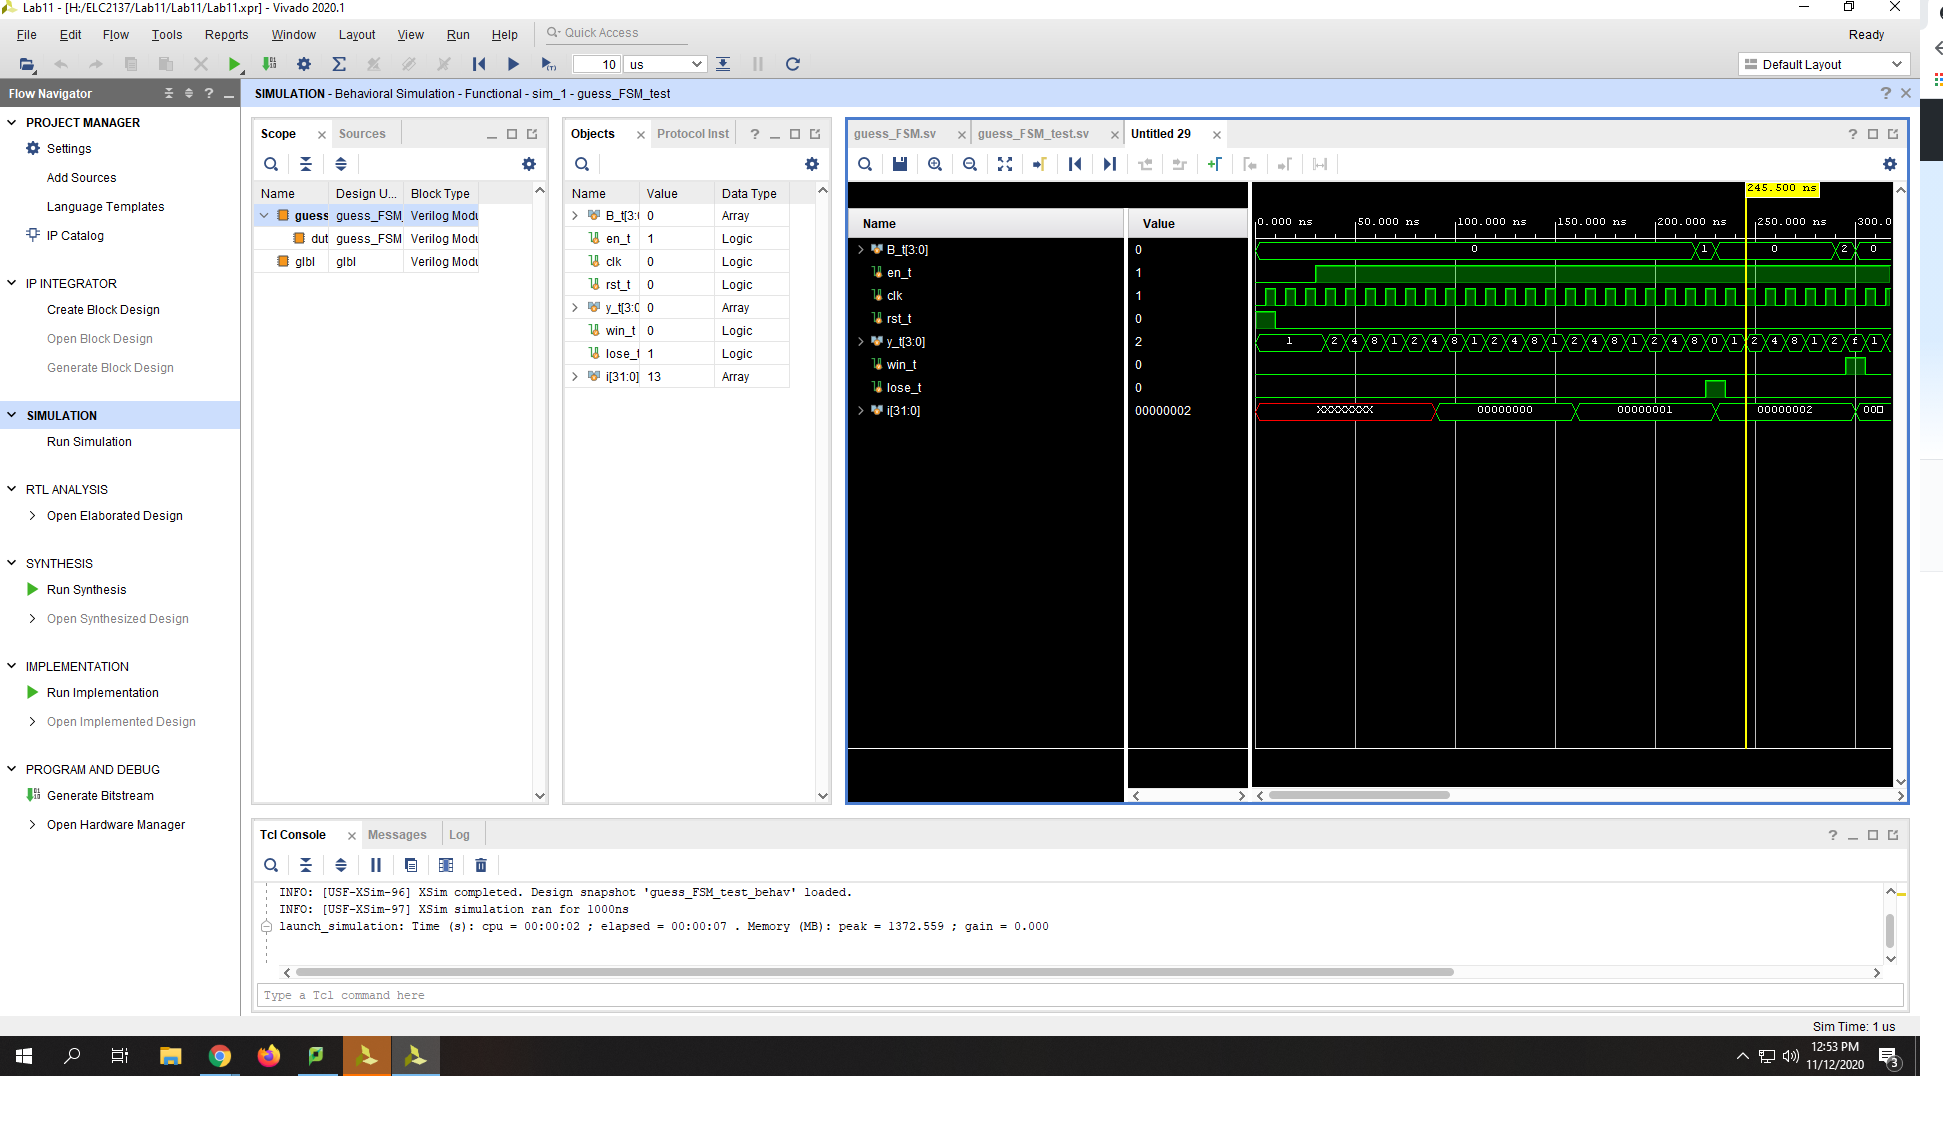
\includegraphics[width=0.8\textwidth]{guess_FSM_sh.PNG}
	
	\item Guessing Game Test Simulation 
	
	%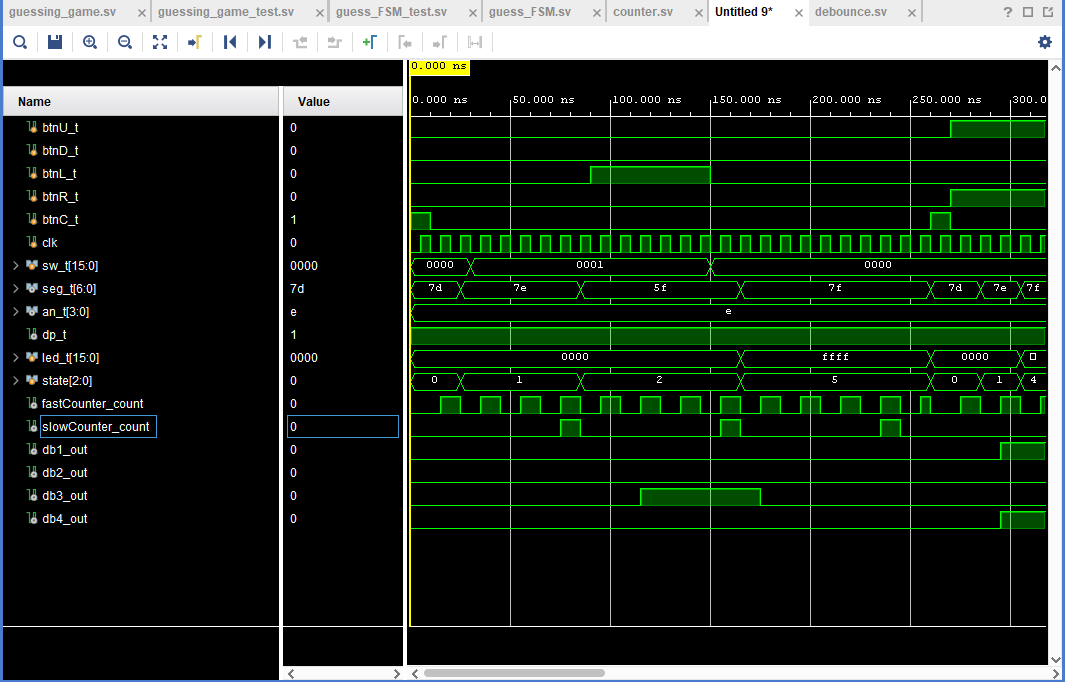
\includegraphics[width=0.8\textwidth]{guessing_game_sc.png}

\end{enumerate}

\section*{Code}

\begin{lstlisting}[style=Verilog,caption=Counter, label=counter.sv]
module counter #(parameter N=1)(
	input clk,
	input rst,
	output tic
	);
	
	wire [N-1:0] Qnext;
	wire [N-1:0] Qreg;
	assign Qnext = Qreg +1;

	register #(.N(N)) my_reg_in_count1(
		.D(Qnext),
		.clk(clk),
		.en(1),
		.rst(rst),
		.Q(Qreg)
	);

	assign tic = &Qreg;
	endmodule
\end{lstlisting}

\begin{lstlisting}[style=Verilog,caption=Guess FSM, label=guess_FSM.sv]
module guess_FSM(
	input [3:0] B,
	input en,
	input clk,
	input rst,
	output reg [3:0] y,
	output reg win,
	output reg lose,
	output reg [15:0] display
	);


	localparam s0    = 3'b000;
	localparam s1    = 3'b001;
	localparam s2    = 3'b010;
	localparam s3    = 3'b011;
	localparam slose = 3'b100;
	localparam swin  = 3'b101;

	// internal signals
	reg [2:0] state, state_next;

	// state memory (register)
	always_ff @(posedge(clk), posedge(rst))
		if (rst) 
			begin
				state <= s0;
			end
		else if(en) 
			begin
				state <= state_next;
			end


	always @*
		case(state)
			s0: 
				if(B == 4'b0000)
					state_next = s1;
				else if (B[3]==1 || B[2]==1 || B[1]==1)
					state_next = slose;
				else 
					state_next = swin;

			s1:
				if(B == 4'b0000)
					state_next = s2;
				else if (B[3]==1 || B[2]==1 || B[0]==1)
					state_next = slose;
				else 
					state_next = swin;

			s2: 
				if(B == 4'b0000)
					state_next = s3;
				else if (B[3]==1 || B[1]==1 || B[0]==1)
					state_next = slose;
				else 
					state_next = swin;
				
			s3: 
				if(B == 4'b0000)
					state_next = s0;
				else if (B[2]==1 || B[1]==1 || B[0]==1)
					state_next = slose;
				else 
					state_next = swin;
			
			swin:
				state_next = swin;
			slose:
				state_next = slose;
		endcase


	always @* 
		begin 
			win = 1'b0;
			lose = 1'b0;
			display = 16'b0;
			case(state)
				s0: y = 4'b0001;
				s1: y = 4'b0010;
				s2: y = 4'b0100;
				s3: y = 4'b1000;
				swin: 
					begin 
					y = 4'b1111;
					win = 1'b1;
					lose = 1'b0;
					display = 16'b1111111111111111; 
				end
					slose: 
					begin 
					y = 4'b0000;
					win = 1'b0;
					lose = 1'b1; 
					display = 16'b1010101010101010;
				end
			endcase
		end

endmodule
\end{lstlisting}

\begin{lstlisting}[style=Verilog,caption=Guess FSM Test, label=guess_FSM_test.sv]
module guess_FSM_test();

	reg [3:0] B_t; 
	reg en_t;
	reg clk;
	reg rst_t;
	reg [3:0] y_t;
	reg win_t;
	reg lose_t;
	integer i;
	
	guess_FSM #(.N(21)) dut(
		.B(B_t),
		.en(en_t),
		.clk(clk),
		.rst(rst_t),
		.y(y_t),
		.win(win_t),
		.lose(lose_t)
		);
	
	always begin 
		clk = ~clk; #5;
	end 

	initial begin   
		clk = 0; rst_t = 1; en_t = 0; B_t = 4'b0000; #10;
		rst_t = 0; #20;
		en_t = 1; #60;
		
		for (i = 0; i <= 4'b1111; i = i + 1) begin 
			B_t = 4'b0000;
			#60;
			B_t = i;
			#10;
		end 
		
		B_t = 4'b0000;
		en_t = 0; #50;
		en_t = 1; #60;
		rst_t = 1; #10;
		rst_t = 0;
		
		for (i = 0; i <= 4'b1111; i = i + 1) begin 
			B_t = 4'b0000;
			#50;
			B_t = i;
			#10;
		end 
		
		B_t = 4'b0000;
		en_t = 0; #50;
		en_t = 1; #60;
		rst_t = 1; #10;
		rst_t = 0;
		
		for (i = 0; i <= 4'b1111; i = i + 1) begin 
			B_t = 4'b0000;
			#70;
			B_t = i;
			#10;
		end 
		
		B_t = 4'b0000;
		en_t = 0; #50;
		en_t = 1; #60;
		rst_t = 1; #10;
		rst_t = 0;
		
		for (i = 0; i <= 4'b1111; i = i + 1) begin 
			B_t = 4'b0000;
			#80;
			B_t = i;
			#10;
		end 
		$finish;
	end 

endmodule
\end{lstlisting}

\begin{lstlisting}[style=Verilog,caption=y decoder, label=y_decoder.sv]
module y_decoder(
	input [3:0] in,
	output reg [6:0] out
	);
	
	always @*
		case (in)
			4'b0001: out = 7'b1111101;
			4'b0010: out = 7'b1111110;
			4'b0100: out = 7'b1011111;
			4'b1000: out = 7'b0111111;
			default: out = 7'b1111111;
		endcase
endmodule
\end{lstlisting}

\begin{lstlisting}[style=Verilog,caption=Guessing Game, label=guessing_game.sv]
module guessing_game #(parameter N = 26, D = 21)(
	input btnU,
	input btnD,
	input btnL,
	input btnR,
	input btnC,
	input clk,
	input [15:0] sw,
	output [6:0] seg,
	output [3:0] an,
	output dp,
	output reg [15:0] led
	);
	
	wire db1_out;
	wire db2_out;
	wire db3_out;
	wire db4_out;
	wire db1_tick;
	wire db2_tick;
	wire db3_tick;
	wire db4_tick;
	wire fastCounter_count;
	wire slowCounter_count;
	wire mux2_out;
	wire [3:0] guess_FSM_y;
	wire guess_FSM_win;
	wire guess_FSM_lose;
	
	debounce #(.N(D))db1(
		.clk(clk),
		.reset(btnC),
		.in(btnU),
		.out(db1_out),
		.tick(db1_tick)
	);
	
	debounce #(.N(D))db2(
		.clk(clk),
		.reset(btnC),
		.in(btnD),
		.out(db2_out),
		.tick(db2_tick)
	);
	
	debounce #(.N(D)) db3(
		.clk(clk),
		.reset(btnC),
		.in(btnL),
		.out(db3_out),
		.tick(db3_tick)
	);
	
	debounce #(.N(D)) db4(
		.clk(clk),
		.reset(btnC),
		.in(btnR),
		.out(db4_out),
		.tick(db4_tick)
	);
	
	counter #(.N(N-2)) fastCounter_game(
		.clk(clk),
		.rst(btnC),
		.tic(fastCounter_count)
	);
	
	counter #(.N(N)) slowCounter_game(
		.clk(clk),
		.rst(btnC),
		.tic(slowCounter_count)
	);
	
	
	mux2 #(.BITS(1)) mux2_guess(
		.in0(fastCounter_count),
		.in1(slowCounter_count),
		.sel(sw[0]),
		.out(mux2_out)
	);
	
	guess_FSM guess_FSM_game(
		.B({db2_out, db3_out, db1_out, db4_out}),
		.en(mux2_out),
		.clk(clk),
		.rst(btnC),
		.y(guess_FSM_y),
		.win(guess_FSM_win),
		.lose(guess_FSM_lose),
		.display(led)
	);
	
	y_decoder guess_y_decoder(
		.in(guess_FSM_y),
		.out(seg)
	);
	
	assign dp = 1'b1;
	assign an = 4'b1110;


endmodule 
\end{lstlisting}

\begin{lstlisting}[style=Verilog,caption=Guessing Game test, label=guessing_game_test.sv]
module guessing_game_test();

	reg btnU_t;
	reg btnD_t;
	reg btnL_t;
	reg btnR_t;
	reg btnC_t;
	reg clk;
	reg [15:0] sw_t;
	wire [6:0] seg_t;
	wire [3:0] an_t;
	wire dp_t;
	reg [15:0] led_t;
	
	guessing_game #(.N(3), .D(1)) dut(
		.btnU(btnU_t),
		.btnD(btnD_t),
		.btnL(btnL_t),
		.btnR(btnR_t),
		.btnC(btnC_t),
		.clk(clk),
		.sw(sw_t),
		.seg(seg_t),
		.an(an_t),
		.dp(dp_t),
		.led(led_t)
	);
	
	
	always begin 
		clk = ~clk; #5;
	end 
	
	initial begin   
		clk = 0; btnC_t = 1; sw_t = 0; btnR_t = 0; 
		btnU_t = 0; btnL_t = 0; btnD_t = 0; #10;
		btnC_t = 0; #20;
		sw_t = 1; #60;
		
		
		btnR_t = 0; btnU_t = 0; 
		btnL_t = 1; btnD_t = 0; #60;
		
		btnR_t = 0; btnU_t = 0; 
		btnL_t = 0; btnD_t = 0; 
		sw_t = 0; #50;
		sw_t = 0; #60;
		btnC_t = 1; #10;
		btnC_t = 0;
		
		btnR_t = 1; btnU_t = 1; 
		btnL_t = 0; btnD_t = 0; #60;
		
		btnR_t = 0; btnU_t = 0; 
		btnL_t = 0; btnD_t = 0; 
		sw_t = 0; #50;
		sw_t = 1; #60;
		btnC_t = 1; #10;
		btnC_t = 0;
		
		btnR_t = 0; btnU_t = 1; 
		btnL_t = 0; btnD_t = 0; #60;
		
		btnR_t = 0; btnU_t = 0; 
		btnL_t = 0; btnD_t = 0; 
		sw_t = 0; #50;
		sw_t = 1; #60;
		btnC_t = 1; #10;
		btnC_t = 0;
		
		btnR_t = 0; btnU_t = 0; 
		btnL_t = 0; btnD_t = 0; #60;
		
		btnR_t = 0; btnU_t = 0; 
		btnL_t = 0; btnD_t = 0; 
		sw_t = 0; #50;
		sw_t = 1; #60;
		btnC_t = 1; #10;
		btnC_t = 0;
		
		btnR_t = 0; btnU_t = 0; 
		btnL_t = 0; btnD_t = 0; #60;
		
		btnR_t = 0; btnU_t = 0; 
		btnL_t = 1; btnD_t = 0; 
		sw_t = 0; #50;
		sw_t = 1; #60;
		btnC_t = 1; #10;
		btnC_t = 0;
		
		btnR_t = 0; btnU_t = 0; 
		btnL_t = 0; btnD_t = 0; #60;
		
		btnR_t = 0; btnU_t = 0; 
		btnL_t = 0; btnD_t = 0; 
		sw_t = 0; #50;
		sw_t = 1; #60;
		btnC_t = 1; #10;
		btnC_t = 0;
		
		btnR_t = 0; btnU_t = 0; 
		btnL_t = 0; btnD_t = 1; #60;
		
		btnR_t = 0; btnU_t = 0; 
		btnL_t = 0; btnD_t = 0; 
		sw_t = 0; #50;
		sw_t = 1; #60;
		btnC_t = 1; #10;
		btnC_t = 0;
		
		btnR_t = 1; btnU_t = 0; 
		btnL_t = 1; btnD_t = 1; #60;
		
		btnR_t = 0; btnU_t = 0; 
		btnL_t = 0; btnD_t = 0; 
		sw_t = 0; #50;
		sw_t = 1; #60;
		btnC_t = 1; #10;
		btnC_t = 0;
		$finish;
	end



endmodule

\end{lstlisting}




\end{document}
